\documentclass[tikz,border=10pt]{standalone}

\usepackage{tikz}
\usetikzlibrary{shapes,arrows,positioning,calc,backgrounds,fit}

% MINIX TikZ style guide color palette
\definecolor{primaryblue}{RGB}{41,128,185}
\definecolor{secondarygreen}{RGB}{39,174,96}
\definecolor{accentorange}{RGB}{230,126,34}
\definecolor{warningred}{RGB}{192,57,43}
\definecolor{lightgray}{RGB}{236,240,241}
\definecolor{darkgray}{RGB}{52,73,94}

\begin{document}
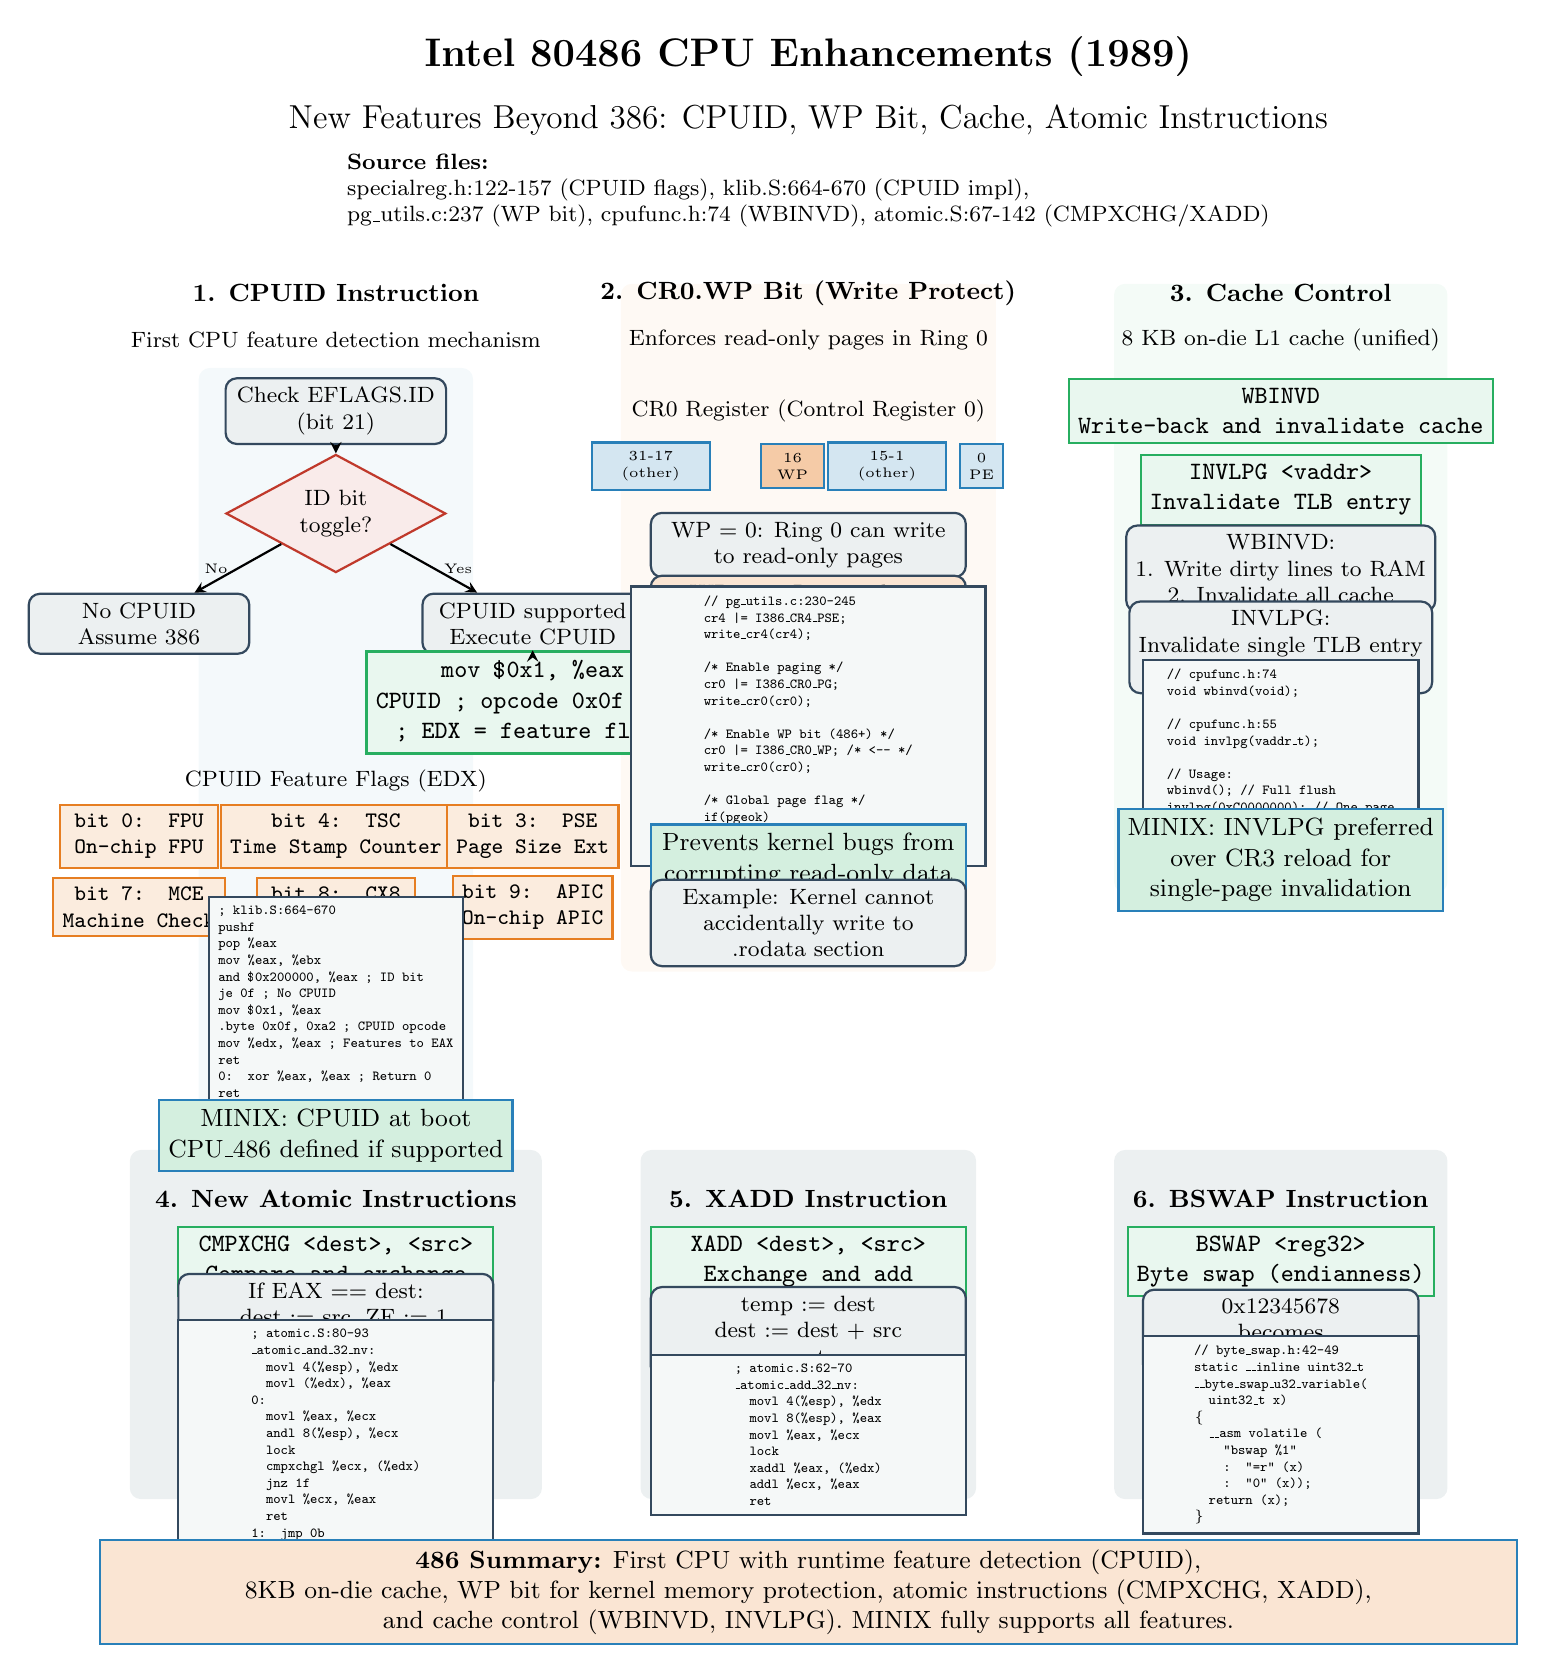
\begin{tikzpicture}[
    % Node styles
    box/.style={rectangle, draw=primaryblue, fill=primaryblue!10, thick, minimum width=2.5cm, minimum height=0.8cm, font=\small, align=center},
    regbox/.style={rectangle, draw=accentorange, fill=accentorange!15, thick, minimum width=2cm, minimum height=0.6cm, font=\footnotesize\ttfamily, align=center},
    instrbox/.style={rectangle, draw=secondarygreen, fill=secondarygreen!10, thick, minimum width=3cm, minimum height=0.7cm, font=\small\ttfamily, align=center},
    flowbox/.style={rectangle, draw=darkgray, fill=lightgray, thick, rounded corners, minimum width=2.8cm, minimum height=0.7cm, font=\footnotesize, align=center},
    decision/.style={diamond, draw=warningred, fill=warningred!10, thick, minimum width=1.5cm, minimum height=1.5cm, font=\footnotesize, align=center, aspect=2},
    label/.style={font=\small\bfseries, align=center},
    arrow/.style={->, >=stealth, thick},
    codebox/.style={rectangle, draw=darkgray, fill=lightgray!50, thick, font=\tiny\ttfamily, align=left, minimum width=3cm},
    bitbox/.style={rectangle, draw=primaryblue, fill=primaryblue!20, thick, minimum height=0.5cm, font=\tiny, align=center},
]

% Title
\node[font=\Large\bfseries] at (10, 21) {Intel 80486 CPU Enhancements (1989)};
\node[font=\large] at (10, 20.2) {New Features Beyond 386: CPUID, WP Bit, Cache, Atomic Instructions};

% Source file references
\node[font=\footnotesize, align=left] at (10, 19.3) {
    \textbf{Source files:}\\
    specialreg.h:122-157 (CPUID flags), klib.S:664-670 (CPUID impl),\\
    pg\_utils.c:237 (WP bit), cpufunc.h:74 (WBINVD), atomic.S:67-142 (CMPXCHG/XADD)
};

% ============================================================================
% SECTION 1: CPUID INSTRUCTION (LEFT COLUMN)
% ============================================================================

\node[label] at (4, 18) {\textbf{1. CPUID Instruction}};
\node[font=\footnotesize, align=center] at (4, 17.4) {First CPU feature detection mechanism};

% CPUID feature detection flow
\node[flowbox] (cpuid_check) at (4, 16.5) {Check EFLAGS.ID\\(bit 21)};
\node[decision] (cpuid_decision) at (4, 15.2) {ID bit\\toggle?};
\node[flowbox] (no_cpuid) at (1.5, 13.8) {No CPUID\\Assume 386};
\node[flowbox] (has_cpuid) at (6.5, 13.8) {CPUID supported\\Execute CPUID};

\draw[arrow] (cpuid_check) -- (cpuid_decision);
\draw[arrow] (cpuid_decision) -- node[left, font=\tiny] {No} (no_cpuid);
\draw[arrow] (cpuid_decision) -- node[right, font=\tiny] {Yes} (has_cpuid);

% CPUID execution box
\node[instrbox] (cpuid_exec) at (6.5, 12.8) {mov \$0x1, \%eax\\CPUID ; opcode 0x0f 0xa2\\; EDX = feature flags};

\draw[arrow] (has_cpuid) -- (cpuid_exec);

% CPUID feature flags (EDX register bits)
\node[label, font=\footnotesize] at (4, 11.8) {CPUID Feature Flags (EDX)};
\node[regbox] (cpuid_fpu) at (1.5, 11.1) {bit 0: FPU\\On-chip FPU};
\node[regbox] (cpuid_tsc) at (4, 11.1) {bit 4: TSC\\Time Stamp Counter};
\node[regbox] (cpuid_pse) at (6.5, 11.1) {bit 3: PSE\\Page Size Ext};

\node[regbox] (cpuid_mce) at (1.5, 10.2) {bit 7: MCE\\Machine Check};
\node[regbox] (cpuid_cx8) at (4, 10.2) {bit 8: CX8\\CMPXCHG8B};
\node[regbox] (cpuid_apic) at (6.5, 10.2) {bit 9: APIC\\On-chip APIC};

% Code example: CPUID implementation from klib.S:664-670
\node[codebox] (cpuid_code) at (4, 9) {
; klib.S:664-670\\
pushf\\
pop \%eax\\
mov \%eax, \%ebx\\
and \$0x200000, \%eax ; ID bit\\
je 0f ; No CPUID\\
mov \$0x1, \%eax\\
.byte 0x0f, 0xa2 ; CPUID opcode\\
mov \%edx, \%eax ; Features to EAX\\
ret\\
0: xor \%eax, \%eax ; Return 0\\
ret
};

% MINIX implementation note
\node[box, fill=secondarygreen!20] at (4, 7.3) {MINIX: CPUID at boot\\CPU\_486 defined if supported};

% ============================================================================
% SECTION 2: CR0.WP BIT (CENTER COLUMN)
% ============================================================================

\node[label] at (10, 18) {\textbf{2. CR0.WP Bit (Write Protect)}};
\node[font=\footnotesize, align=center] at (10, 17.4) {Enforces read-only pages in Ring 0};

% CR0 register with WP bit highlighted
\node[label, font=\footnotesize] at (10, 16.5) {CR0 Register (Control Register 0)};

% CR0 bit layout (simplified, focus on WP bit)
\node[bitbox, minimum width=1.5cm] at (8, 15.8) {31-17\\(other)};
\node[bitbox, minimum width=0.8cm, fill=accentorange!40] at (9.8, 15.8) {16\\WP};
\node[bitbox, minimum width=1.5cm] at (11, 15.8) {15-1\\(other)};
\node[bitbox, minimum width=0.5cm] at (12.2, 15.8) {0\\PE};

% WP bit explanation
\node[flowbox, minimum width=4cm] at (10, 14.8) {WP = 0: Ring 0 can write\\to read-only pages};
\node[flowbox, minimum width=4cm, fill=accentorange!20] at (10, 14) {WP = 1: Ring 0 obeys\\read-only protection};

% Code example: WP bit enablement from pg_utils.c:237
\node[codebox, minimum width=4.5cm] (wp_code) at (10, 12.5) {
// pg\_utils.c:230-245\\
cr4 |= I386\_CR4\_PSE;\\
write\_cr4(cr4);\\
\\
/* Enable paging */\\
cr0 |= I386\_CR0\_PG;\\
write\_cr0(cr0);\\
\\
/* Enable WP bit (486+) */\\
cr0 |= I386\_CR0\_WP; /* <-- */\\
write\_cr0(cr0);\\
\\
/* Global page flag */\\
if(pgeok)\\
\ \ \ \ cr4 |= I386\_CR4\_PGE;\\
write\_cr4(cr4);
};

% WP benefit
\node[box, fill=secondarygreen!20, minimum width=4cm] at (10, 10.8) {Prevents kernel bugs from\\corrupting read-only data};

% Use case
\node[flowbox, minimum width=4cm] at (10, 10) {Example: Kernel cannot\\accidentally write to\\.rodata section};

% ============================================================================
% SECTION 3: CACHE CONTROL (RIGHT COLUMN)
% ============================================================================

\node[label] at (16, 18) {\textbf{3. Cache Control}};
\node[font=\footnotesize, align=center] at (16, 17.4) {8 KB on-die L1 cache (unified)};

% Cache instructions
\node[instrbox] (wbinvd_instr) at (16, 16.5) {WBINVD\\Write-back and invalidate cache};
\node[instrbox] (invlpg_instr) at (16, 15.5) {INVLPG <vaddr>\\Invalidate TLB entry};

% WBINVD explanation
\node[flowbox, minimum width=3.5cm] at (16, 14.5) {WBINVD:\\1. Write dirty lines to RAM\\2. Invalidate all cache};

% INVLPG explanation
\node[flowbox, minimum width=3.5cm] at (16, 13.5) {INVLPG:\\Invalidate single TLB entry\\(faster than full flush)};

% Code reference
\node[codebox, minimum width=3.5cm] at (16, 12.3) {
// cpufunc.h:74\\
void wbinvd(void);\\
\\
// cpufunc.h:55\\
void invlpg(vaddr\_t);\\
\\
// Usage:\\
wbinvd(); // Full flush\\
invlpg(0xC0000000); // One page
};

% MINIX usage
\node[box, fill=secondarygreen!20, minimum width=3.5cm] at (16, 10.8) {MINIX: INVLPG preferred\\over CR3 reload for\\single-page invalidation};

% ============================================================================
% SECTION 4: NEW ATOMIC INSTRUCTIONS (BOTTOM LEFT)
% ============================================================================

\node[label] at (4, 6.5) {\textbf{4. New Atomic Instructions}};

% CMPXCHG instruction
\node[instrbox, minimum width=4cm] (cmpxchg) at (4, 5.7) {CMPXCHG <dest>, <src>\\Compare and exchange};

\node[flowbox, minimum width=4cm] at (4, 4.8) {If EAX == dest:\\\ \ dest := src, ZF := 1\\Else:\\\ \ EAX := dest, ZF := 0};

% Code example: CMPXCHG from atomic.S:87
\node[codebox, minimum width=4cm] at (4, 3.5) {
; atomic.S:80-93\\
\_atomic\_and\_32\_nv:\\
\ \ movl 4(\%esp), \%edx\\
\ \ movl (\%edx), \%eax\\
0:\\
\ \ movl \%eax, \%ecx\\
\ \ andl 8(\%esp), \%ecx\\
\ \ lock\\
\ \ cmpxchgl \%ecx, (\%edx)\\
\ \ jnz 1f\\
\ \ movl \%ecx, \%eax\\
\ \ ret\\
1: jmp 0b
};

% ============================================================================
% SECTION 5: XADD INSTRUCTION (BOTTOM CENTER)
% ============================================================================

\node[label] at (10, 6.5) {\textbf{5. XADD Instruction}};

% XADD instruction
\node[instrbox, minimum width=4cm] (xadd) at (10, 5.7) {XADD <dest>, <src>\\Exchange and add};

\node[flowbox, minimum width=4cm] at (10, 4.8) {temp := dest\\dest := dest + src\\src := temp};

% Code example: XADD from atomic.S:67
\node[codebox, minimum width=4cm] at (10, 3.5) {
; atomic.S:62-70\\
\_atomic\_add\_32\_nv:\\
\ \ movl 4(\%esp), \%edx\\
\ \ movl 8(\%esp), \%eax\\
\ \ movl \%eax, \%ecx\\
\ \ lock\\
\ \ xaddl \%eax, (\%edx)\\
\ \ addl \%ecx, \%eax\\
\ \ ret
};

% ============================================================================
% SECTION 6: BSWAP INSTRUCTION (BOTTOM RIGHT)
% ============================================================================

\node[label] at (16, 6.5) {\textbf{6. BSWAP Instruction}};

% BSWAP instruction
\node[instrbox, minimum width=3.5cm] (bswap) at (16, 5.7) {BSWAP <reg32>\\Byte swap (endianness)};

\node[flowbox, minimum width=3.5cm] at (16, 4.8) {0x12345678\\becomes\\0x78563412};

% Code example: BSWAP from byte_swap.h:46
\node[codebox, minimum width=3.5cm] at (16, 3.5) {
// byte\_swap.h:42-49\\
static \_\_inline uint32\_t\\
\_\_byte\_swap\_u32\_variable(\\
\ \ uint32\_t x)\\
\{\\
\ \ \_\_asm volatile (\\
\ \ \ \ "bswap \%1"\\
\ \ \ \ : "=r" (x)\\
\ \ \ \ : "0" (x));\\
\ \ return (x);\\
\}
};

% ============================================================================
% BOTTOM SUMMARY
% ============================================================================

\node[box, fill=accentorange!20, minimum width=18cm, minimum height=1.2cm] at (10, 1.5) {
\textbf{486 Summary:} First CPU with runtime feature detection (CPUID),\\
8KB on-die cache, WP bit for kernel memory protection, atomic instructions (CMPXCHG, XADD),\\
and cache control (WBINVD, INVLPG). MINIX fully supports all features.
};

% Coordinate anchors for background zones
\coordinate (wp_top) at (8, 18);
\coordinate (wp_bottom) at (12, 9.5);
\coordinate (cache_top) at (14, 18);
\coordinate (cache_bottom) at (18, 10.5);
\coordinate (atomic1_top) at (1.5, 7);
\coordinate (atomic1_bottom) at (6.5, 2.8);
\coordinate (atomic2_top) at (8, 7);
\coordinate (atomic2_bottom) at (12, 2.8);
\coordinate (atomic3_top) at (14, 7);
\coordinate (atomic3_bottom) at (18, 2.8);

% Background zones
\begin{pgfonlayer}{background}
    % CPUID section background
    \node[fill=primaryblue!5, rounded corners, fit=(cpuid_check) (cpuid_code)] {};

    % WP bit section background
    \node[fill=accentorange!5, rounded corners, fit=(wp_top) (wp_code) (wp_bottom)] {};

    % Cache section background
    \node[fill=secondarygreen!5, rounded corners, fit=(cache_top) (invlpg_instr) (cache_bottom)] {};

    % Atomic instructions section background
    \node[fill=lightgray, rounded corners, fit=(atomic1_top) (cmpxchg) (atomic1_bottom)] {};
    \node[fill=lightgray, rounded corners, fit=(atomic2_top) (xadd) (atomic2_bottom)] {};
    \node[fill=lightgray, rounded corners, fit=(atomic3_top) (bswap) (atomic3_bottom)] {};
\end{pgfonlayer}

\end{tikzpicture}
\end{document}
